% ==================== Header ====================
\documentclass[12pt]{article} %montserrat fonts exists only in 10pt-12pt
\usepackage[a4paper, top=10mm, bottom=10mm, left=12mm, right=12mm]{geometry}
\usepackage[most]{tcolorbox}
\usepackage[hidelinks]{hyperref}
\usepackage[defaultfam,tabular,lining]{montserrat}
\usepackage{enumitem}
\usepackage{dirtytalk}
\usepackage{fontawesome5}
\usepackage{numprint}
\usepackage{setspace}

% ==================== Global settings ====================
\npdecimalsign{,} % Comma for decimals (European style)
\npthousandsep{.} % Dot for thousands (European style)
\setlength{\parindent}{0mm} % No paragraph indent
\pagenumbering{gobble} % No page numbering
\hyphenpenalty=100000 % No implicit hyphens
\exhyphenpenalty=100000 % No explicit hyphens
\tolerance=5000 % Avoid bad spacing
\emergencystretch=1em % Allow minor overshoots (trust me, looks better)

% ==================== Custom commands ====================
\definecolor{custom_blue}{RGB}{2,132,199}

\definecolor{linkedin_blue}{RGB}{10,102,194}

\newcommand{\NameText}[1] {{\Large\textbf{#1}}}

\newcommand{\HighlightedText}[1] {{\textbf{#1}}}

\newcommand{\PlaceAndTime}[2] {\HighlightedText{#1} \hfill \HighlightedText{#2}}

\newcommand{\SymbolAndLink}[3] {#1 \hspace{0mm} \href{#3} {\underline{#2}}}

\newcommand{\SymbolAndText}[2] {#1 \hspace{0mm} #2}

\newenvironment{ItemizeSection}[1]{
    \vspace{1mm}
    \HighlightedText{#1}
    \vspace{0.5mm}
    {\color{custom_blue} \hrule}
    \begin{itemize}[left=0.5em, topsep=0pt, itemsep=0pt, label={$\bullet$}]
}{
    \end{itemize}
}

\newenvironment{TextSection}[1]{
    \vspace{1mm}
    \HighlightedText{#1}
    \vspace{0.5mm}
    {\color{custom_blue} \hrule}
    \begin{itemize}[left=0.5em, topsep=0pt, itemsep=0pt, label={}]
}{
    \end{itemize}
}

\newenvironment{ItemizeSubsection}{
    \begin{itemize}[left=0.5em, topsep=-999pt, itemsep=0pt, label={$\circ$}]
}{
    \end{itemize}
}

% ==================== Name and Contact ====================

\begin{document}
\setstretch{1.5} % Spacing for the header
\begin{tcolorbox}[sharp corners=all, colback=custom_blue, coltext=white, frame empty, left=2mm, right=2mm, top=1mm, bottom=1mm]

    \noindent \begin{minipage}{0.6\textwidth}
        \NameText{Kyrylo Sovailo}

        \SymbolAndLink{\faAt}{k.sovailo@gmail.com}{mailto:k.sovailo@gmail.com} \\
        \SymbolAndLink{\faPhone*}{01763 5479038}{tel:+4917635479038} \\
        %\SymbolAndLink{\faGithub}{github.com}{https://github.com/kyrylo-sovailo} \\
        \SymbolAndLink{\faLinkedin}{linkedin.com}{https://linkedin.com/in/kyrylo-sovailo-19b4541b9} \\
        \SymbolAndText{\faEnvelope}{Pallaswiesenstr. 39, 64293 Darmstadt} \\
        %\SymbolAndText{\faAddressCard}{Citisenship: Ukraine} \\
        %\SymbolAndText{\faBabyCarriage}{Born at 08.10.2000 in Kiew, Ukraine} \\
        \SymbolAndText{\faBabyCarriage}{Born at 08.10.2000}

    \end{minipage}
    \begin{minipage}{0.39\textwidth}
        \raggedleft
        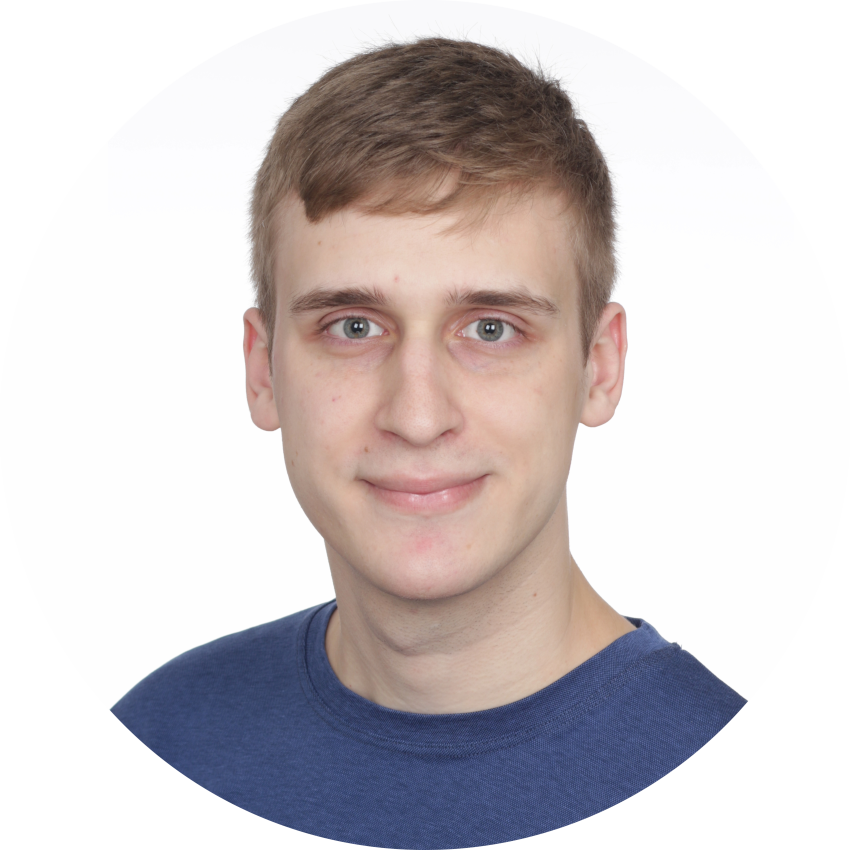
\includegraphics[width=50mm]{Photo_compressed_round.png}
    \end{minipage}
\end{tcolorbox}
\setstretch{1.1} % Spacing for the rest of the document

% ==================== Summary ====================

\vspace{-2.5mm}
\begin{TextSection}{Profile}
\item Reliable and meticulous employee with a completed Master's degree and experience in software development and related fields. I enjoy working with industrial and scientific equipment but am also willing to learn new skills.
\end{TextSection}

% ==================== Education ====================
\begin{ItemizeSection}{Education}
    \item \PlaceAndTime{Computational Engineering (CE) M.Sc.}{04.2023 -- 12.2025} \\
    \textbf{(Specialization Computational Robotics)} \\
    TU Darmstadt \\
    Final grade: \numprint{2.1} \\
    Thesis grade: \numprint{1.7}

    \item \PlaceAndTime{Computational Engineering Science (CES) B.Sc.}{10.2018 -- 04.2023} \\
    RWTH Aachen University \\
    Final grade: \numprint{2.4} \\
    Thesis grade: \numprint{1.7}

    \item \PlaceAndTime{High school}{09.2017 -- 09.2018} \\
     Studienkolleg at Free University Berlin, technical course
\end{ItemizeSection}

% ==================== Professional background ====================
\begin{ItemizeSection}{Professional experience}
    \item \PlaceAndTime{Student assistant at Goethe University Frankfurt}{06.2023 -- 07.2024} \\
    Buchmann Institute for Molecular Life Sciences (BMLS)
    \begin{ItemizeSubsection}
        \item Software design and development, adapting the software to the new hardware
        \item Handling laboratory equipment
        \item Iterative work, interpreting user feedback
    \end{ItemizeSubsection}

    \item \PlaceAndTime{Intern at Continental AG}{03.2022 -- 05.2022}
    \begin{ItemizeSubsection}
        \item Software development, workflow automation
        \item Work experience in a corporate environment
    \end{ItemizeSubsection}

    \item \PlaceAndTime{Student assistant at RWTH Aachen University}{04.2021 -- 12.2021} \\
    Institute for Data Science in Mechanical Engineering (DSME)
    \begin{ItemizeSubsection}
        \item Commissioning and testing of a robot arm
        \item Development of the software for the robot arm
        \item Supporting PhD students in their research
    \end{ItemizeSubsection}
\end{ItemizeSection}

\newpage
% ==================== Skills ====================
\begin{ItemizeSection}{Skills}
    \item Advanced computer skills
    \item Software development
    \item Basic knowledge of hardware development (CAD, PCB design)
    \item Experience with robots and safety protocols
    \item Soldering, knowledge of electrical and electronic systems
    \item Experience with tools and equipment (saws, drills, small tools)
\end{ItemizeSection}

\begin{ItemizeSection}{Personal strengths}
    \item Reliable and responsible
    \item Meticulous and conscientious work ethic
    \item Ability to work independently and as part of a team
    \item High willingness to learn
\end{ItemizeSection}

\begin{ItemizeSection}{Languages}
    \item Native: Ukrainian
    \item Fluent (C1): German, English
\end{ItemizeSection}

\begin{ItemizeSection}{Further information}
    \item Driving License: B1
\end{ItemizeSection}

\end{document}
